%
% $Id: IIR.tex 14 2014-02-04 22:36:30Z nicb $
%

\svnInfo $Id: IIR.tex 14 2014-02-04 22:36:30Z nicb $

\chapter{Filtri a feedback (IIR)\label{chap:iir}}

\section{Introduzione}

I filtri a feedback (IIR - per \emph{Infinite Impulse Response}) sono filtri nei quali vengono re-immessi in ingresso
versioni ritardate e riscalate dell'uscita.

Il filtro IIR pi\`u semplice \`e:

  \begin{equation}\label{eqn:filtro iir semplice}
		y_t = x_t + a_1 y_{t-1}
	\end{equation}

	In eq.\ref{eqn:filtro iir semplice} l'ultimo campione in uscita viene
	riscalato di un fattore $a_1$ e sommato di nuovo all'ingresso.

Potenzialmente la risposta di questo filtro a un impulso unitario \`e
infinita: p.es., introducendo un segnale consistente in un 1 al campione zero e zero
per tutti gli altri campioni all'interno di un filtro del genere con un
fattore $a_1 = 0.5$ otterremo in uscita:

  \begin{equation}
		y_t = 1, 0.5, 0.25, 0.125, 0.0625, \ldots
  \end{equation}

e cio\`e una risposta \emph{infinita}. Questo non pu\`o mai succedere con i
filtri FIR, la cui risposta \`e al massimo il numero dei campioni in ingresso
pi\`u il numero di campioni del filtro (i \emph{termini} meno uno.

L'altra differenza grossa con i filtri FIR \`e che gli IIR possono
letteralmente \emph{esplodere}. Per capire questo riprendiamo il filtro descritto in
\ref{eqn:filtro iir semplice} e poniamo il fattore $a_1 = 2$. L'uscita
numerica del
filtro sarà:

  \begin{equation}
		y_t = 1, 2, 4, 8, 16, \ldots
  \end{equation}

Essa diverger\`a all'infinito.

Per capire bene perch\'e, sostituiamo in eq.\ref{eqn:filtro iir semplice} a $y_t$ e $x_t$ (singoli campioni) i
vettori $Y$ e $X$ (che rappresentano ``interi segnali''):

  \begin{equation}\label{eqn:filtro iir segnali}
		Y = X + a_1 z^{-1} Y
	\end{equation}

	Se raggruppiamo i termini, l'eq.\ref{eqn:filtro iir segnali} diventa:

  \begin{equation}\label{eqn:filtro iir segnali raggruppata}
		X = Y - a_1 z^{-1} Y
	\end{equation}

Ma questa \`e l'equazione dei filtri FIR (feed--forward), solo che ingressi e
uscite sono scambiati. Sappiamo che la funzione di trasferimento del
corrispondente filtro FIR \`e:

	\begin{equation}
		1 - a_1 z^{-1}
	\end{equation}

e, dato che il caso del filtro IIR presenta l'equazione in forma invertita,
ossia:

	\begin{equation}
		X = H(z) Y
	\end{equation}

ovvero

	\begin{equation}
		Y = \frac{1}{H(z)} X
	\end{equation}

la funzione di trasferimento sar\`a quindi:

	\begin{equation}\label{eqn:iir tf}
		H(z) = \frac{1}{1 - a_1 z^{-1}}
	\end{equation}

La magnitudine della risposta in frequenza si otterr\`a come sempre
operando la sostituzione $z = e^{i\omega}$ e calcolando il modulo:

	\begin{equation}\label{eqn:iir tf 2}
		|H(z)| = \frac{1}{|1 - a_1 e^{-i\omega}|}
	\end{equation}

Quando $z = a_1$, $z^{-1} = \frac{1}{a_1}$, il denominatore
dell'eq.\ref{eqn:iir tf 2} diventa

	\begin{equation}\label{eqn:iir tf zero condition}
		1 - \frac{a_1}{a_1} = 1 - 1 = 0
	\end{equation}

e quindi in $a_1$ noi abbiamo un punto che diverge all'infinito. Quel punto si
chiama \emph{polo}.

Per calcolare bene la magnitudine della risposta sar\`a opportuno moltiplicare
numeratore e denominatore per $z$:

	\begin{equation}
		H(z) = \frac{1}{1 - a_1 z^{-1}} = \frac{z}{z - a_1}
	\end{equation}

Il modulo sar\`a

	\begin{equation}
		|H(z)| = \frac{|z|}{|z - a_1|}
	\end{equation}

	oss\`ia, sostituendo $z = e^{i\omega}$

	\begin{equation}\label{eqn:iir tf mag subst}
		|H(z)| = \frac{|e^{i\omega}|}{|e^{i\omega} - a_1|}
	\end{equation}

ma $|e^{i\omega}| = 1$ per qualsiasi $\omega$, quindi l'eq.\ref{eqn:iir tf mag subst}
diventa:

	\begin{equation}\label{eqn:iir tf mag subst no num}
		|H(z)| = \frac{1}{|e^{i\omega} - a_1|}
	\end{equation}

Scomponendo il denominatore in parte reale e parte immaginaria otteniamo

	\begin{equation}
		\begin{array}{l c l}
			Re_{den} & = & cos \omega - a_1\\
			Im_{den} & = & sin \omega\\
		\end{array}
	\end{equation}

e il modulo sar\`a quindi

	\begin{equation}
		|den| = \sqrt{( cos \omega - a_1 )^2 + ( sin \omega )^2}
	\end{equation}

ma

	\begin{equation}
		( cos \omega - a_1 )^2 = ( cos \omega - a_1 ) ( cos \omega - a_1 ) = cos^2 ( \omega ) - 2 a_1 cos ( \omega ) + a_1^2
	\end{equation}

e quindi

	\begin{equation}
		|den| = \sqrt{cos^2 ( \omega ) - 2 a_1 cos ( \omega ) + a_1^2 + sin^2 ( \omega )}
	\end{equation}

Ricordando che $cos^2 + sin^2 = 1$ per qualsiasi $\omega$, possiamo
semplificare:

	\begin{equation}
		|den| = \sqrt{1 - 2 a_1 cos ( \omega ) + a_1^2}
	\end{equation}

e l'eq.\ref{eqn:iir tf mag subst no num} diventa:

	\begin{equation}
		|H(z)| = \frac{1}{\sqrt{1 - 2 a_1 cos ( \omega ) + a_1^2}}
	\end{equation}

	\begin{figure}[htb]
		\begin{center}
			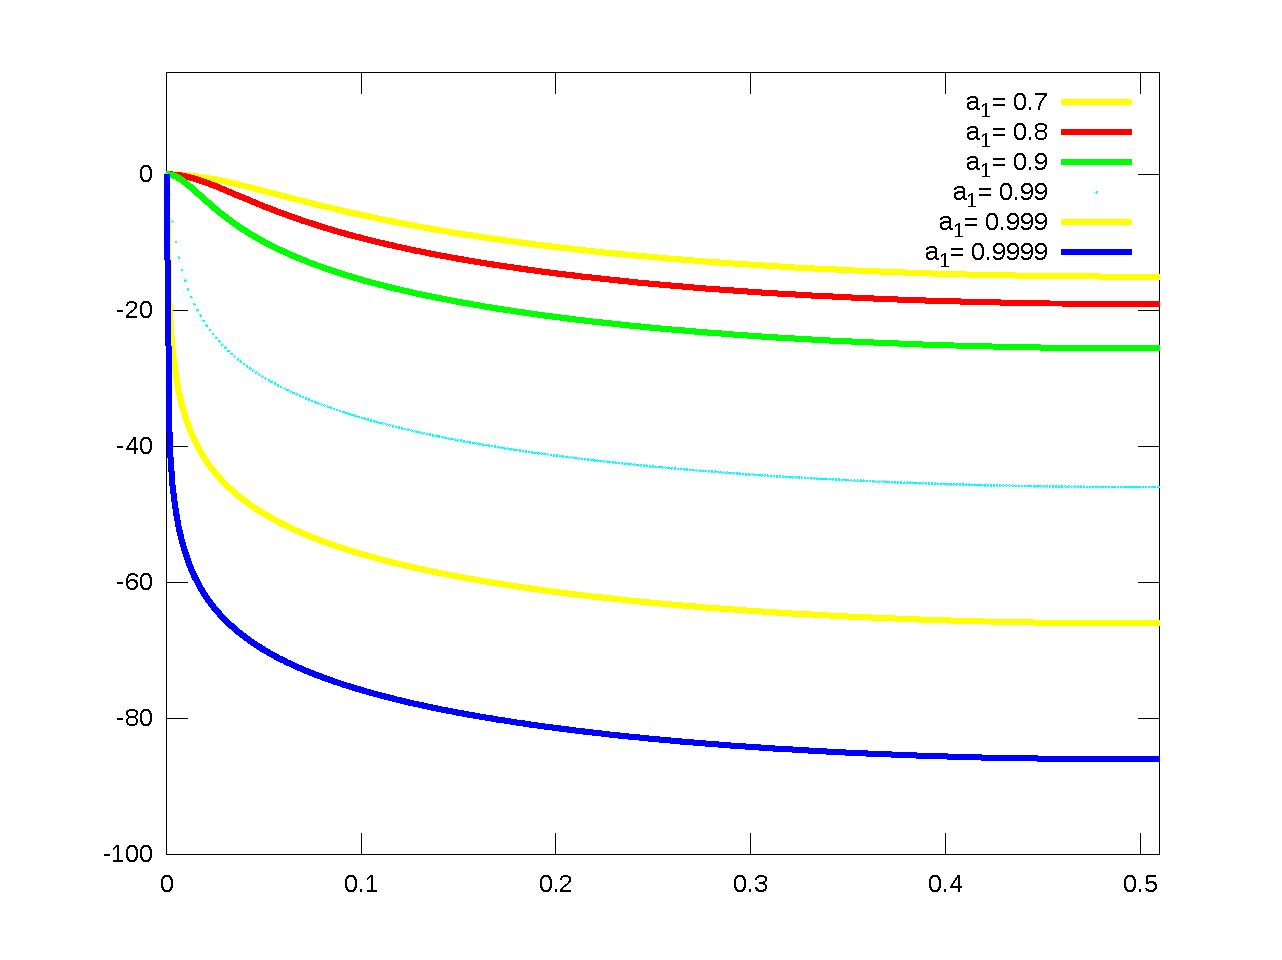
\includegraphics[width=0.6\textwidth]{\plotdir/iir3}
			\caption{Magnitudine (normalizzata a $0 dB$) del filtro IIR $\frac{1}{1 - a_1 z^{-1}}$\label{fig:simple IIR mag response}}
		\end{center}
	\end{figure}

	La figura \vref{fig:simple IIR mag response} illustra la magnitudine
	(normalizzata a $0 dB$) del nostro filtro con valori diversi di $a_1$.

\section{Risonanza e larghezza di banda\label{sec:resonance}}

\subsection{Risonanza e larghezza di banda di un filtro}
Dato che si tratta di una funzione continua, la larghezza di banda di un
  filtro \`e per definizione il punto in cui la potenza \`e dimezzata (cio\`e
	$1/\sqrt{2} = -3 dB$ -- cf.Fig.\vref{fig:bw})

	\begin{figure}[htb]
		\begin{center}
		  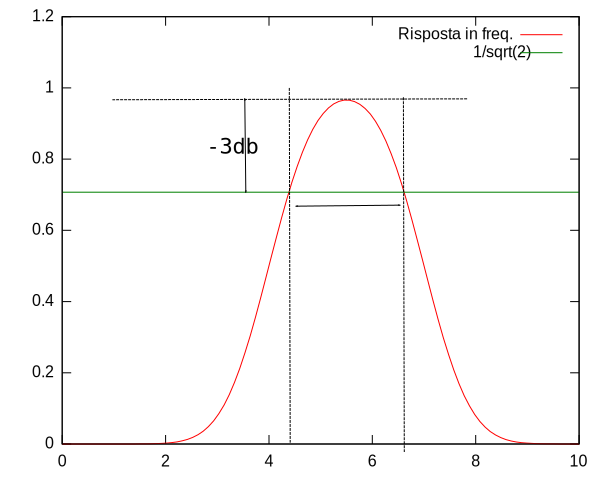
\includegraphics[width=0.6\textwidth]{\imagedir/bw}
		  \caption{Misurazione della larghezza di banda di un filtro\label{fig:bw}}
		\end{center}
	\end{figure}

	Quando un filtro ha un polo collocato da qualche parte sul piano $z$ questo
    polo avr\`a un modulo R e un angolo $\theta$.
  
	Consideriamo ora l'effetto di un polo sul cerchio unitario sull'asse reale:
    se $\theta$ \`e 0 avremo un filtro passa basso e l'algebra si semplifica. Se
    $\theta$ \`e non-zero l'effetto sar\`a uguale ruotato di un angolo
		$\theta$.
  
	Dato che per i fitri IIR a un polo la funzione di trasferimento \`e
  
		 \begin{equation}
				H(z) = \frac{1}{1 - a_1 z^{-1}}
		 \end{equation}

	l'inverso del quadrato della della risposta in magnitudine ad una frequenza
    $\psi (rad/campione)$ legata a questo polo sull'asse reale laddove $z = R$ \`e
  
		 \begin{equation}
				\frac{1}{|H(z)|^2} = |1 - a_1 z^{-1}|^2 = | z - a_1 |^2
		 \end{equation}
  
    ponendo $z = e^{i\theta}$ e $a_1 = R$
  
		 \begin{equation}
				\frac{1}{|H(z)|^2} =  |e^{i\theta} - R|^2
		 \end{equation}
  
    svolgendo il modulo
  
		 \begin{equation}
				\frac{1}{|H(z)|^2} =  1 - 2 R cos\,\theta + R^2
		 \end{equation}
  
	Nel centro della risonanza $\theta = 0$, $cos\,\theta = 1$ e l'equazione diventa:
  
		 \begin{equation}
				\frac{1}{|H(z)|^2} =  1 - 2 R cos\,\theta + R^2
		 \end{equation}

		 \begin{equation}
				\frac{1}{|H(z)|^2} =  1 - 2 R + R^2 = (1 - R)^2
		 \end{equation}

		cio\`e il quadrato della distanza tra
    la frequenza zero sul cerchio unitario $(z = 1)$ \`e il polo
  
  Per trovare i punti in cui la magnitudine \`e $1/\sqrt{2}$, guardiamo
    per quale $\theta$ la magnitudine \`e il doppio di questo, quindi:
  
		\begin{equation}\label{eqn:theta solution for bw}
    1 - 2 R cos \theta + R^2 = 2 (1 - R)^2 = 2 [ 1 - 2R + R^2 ]
		 \end{equation}
  
	Risolviamo quindi l'eq.\ref{eqn:theta solution for bw} per $\theta$:

	\begin{equation}
		- 2 R cos \theta = 2 - 4R + 2 R^2 - 1 - 2 R^2 = 1 - 4 R 
  \end{equation}

	ossia

	\begin{equation}
					cos \theta = -\frac{1}{2 R} + \frac{4 R}{2 R} = - \frac{1}{2R} + 2 R
  \end{equation}

	quindi

	\begin{equation}
		\theta = arccos \left ( 2 R  - \frac{1}{2 R} \right )
	\end{equation}

	%
	% VERIFICARE e inventare un PLOT che faccia vedere
	%
  
\section{Resons}
  
					I filtri a un polo hanno i poli e gli zeri che si dispongono
    soltanto a freq. zero o nyquist, a seconda del fatto che il polo sia pi\`u
    vicino a $z = +1$ o $z = -1$.
  
	Per avere filtri che risuonino ad una frequenza desiderata qualsiasi abbiamo
    (e per fare in modo che il filtro tiri fuori un segnale reale) ci vogliono
    almeno un paio di poli disposti in maniera complessa coniugata
  
		 \begin{equation}
						 H(z) = \frac{1}{(1 - Re^{i\theta} z^{-1})(1 - Re^{-i\theta} z^{-1})}
		 \end{equation}
  
    dove R \`e il modulo del polo e $\theta$ \`e l'angolo (frq) e $Re^{+/-\theta}$ sono le
    radici del denominatore (poli)
  
	Ora se eseguiamo la moltiplicazione del denominatore quello che otteniamo \`e:
  
		 \begin{equation}
			 \begin{array}{r c c c l c l}
     den & = & (1 & - & Re^{i\theta} z^{-1})(1 - Re^{-i\theta} z^{-1}) & &\\
         & = & 1 & - & Re^{-i\theta} z^{-1} - Re^{i\theta} z^{-1} & + & R^{2} z^{-2}\\
         & = & 1 & - & Rz^{-1} (e^{i\theta} + e^{-i\theta}) & + & R^{2} z^{-2}\\
         & = & 1 & - & Rz^{-1} 2 cos \theta & + & R^{2} z^{-2}\\
		 		\end{array}
		 \end{equation}
  
		 \begin{equation}
			 H(z) = \frac{1}{1 - (2R cos \theta) z^{-1} + R^{2} z^{-2}}
		 \end{equation}
  
   
	Se interpretiamo $z^{-1}$ come ``ritardo di un campione'', vediamo subito che
    questa funzione di trasferimento corrisponde al filtro:
  
		 \begin{equation}
    y_t = x_t + (2Rcos \theta) y_{t-1} - R^{2} y_{t-2}
		 \end{equation}
  
% \section{Determinazione della frequenza di un reson}
% 
%  	Per determinare la frequenza di risonanza del reson non si pu\`o prendere
%      direttamene $\theta$ perch\'e l'altro polo influenza la posizione del picco, e
%      quando i poli sono vicini lo shift \`e significativo
%    
%  	Adottiamo un approccio semplicistico: valutiamo la risposta in frequenza come funzione
%      della variabile di frequenza $\psi$ e poi troviamo la frequenza $\psi$ per cui la
%      derivata \`e zero. Per semplificare ulteriormente non prenderemo in
%      considerazione la magnitudine della frequenza, ma il quadrato del suo
%      inverso -- dato che la risposta in frequenza originale ha un massimo
% 		 proprio dove il quadrato del suo inverso ha un minimo
% 		 (cf.\vref{fig:inverse fr})
% 	\begin{figure}[htb]
% 		\begin{center}
% 			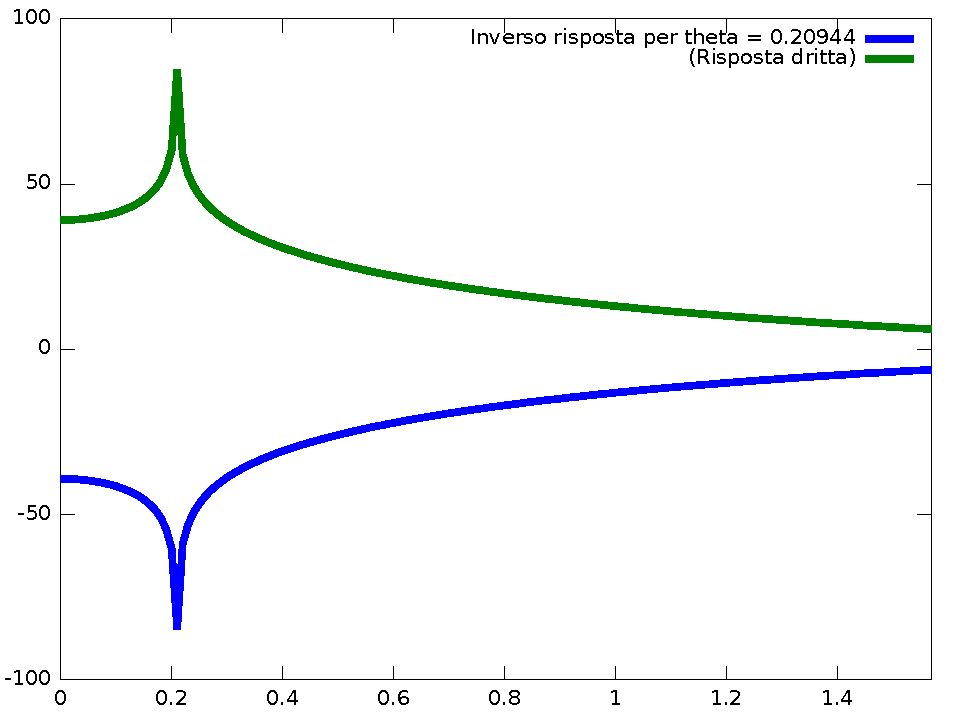
\includegraphics[width=0.6\textwidth]{\plotdir/inverse_fr}
% 			\caption{Inverso della risposta in frequenza per $\theta = \pi/15$ (confrontato col suo dritto)\label{fig:inverse fr}}
% 		\end{center}
% 	\end{figure}
% 
%    
%  	Riprendiamo il quadrato dell'inverso del modulo di $H(z)$:
%    
%  		 \begin{equation}
%      |(1 - Re^{i\theta} z^{-1})(1 - Re^{-i\theta} z^{-1})|^2
%  		 \end{equation}
%    
%    - questa volta conviene moltiplicare tutto per $z^2$ per ottenere la posizione dei
%      poli (dato che $z^2 = 1$ sul cerchio unitario, possiamo farlo)
%    
%  		 \begin{equation}
%      |(z - Re^{i\theta})(z - Re^{-i\theta})|^2
%  		 \end{equation}
%    
%    - sostituiamo $z = e^{i\theta}$
%    
%  		 \begin{equation}
%       |(e^{i\theta} - R e^{i\theta})(e^{i\theta} - Re^{-i\theta})|^2
%  		 \end{equation}
%    
%    % COMPLETARE

\section{Per migliorare i reson: aggiungere gli zeri}

Combinando \emph{feedback} (filtri a poli) con \emph{feed-forward} (filtri
FIR, con zeri) si migliora sostanzialmente la risposta dei filtri Reson
(ed è così che sono fatti normalmente). Questo permette di avere delle buone
risposte anche quando la campana del filtro \`e a bassa frequenza.

Un modo per migliorare la forma \`e quello di porre uno zero a $z = 1$, e
gi\`a che ci siamo per simmetria porne uno anche per $z = nyquist = \pi$.

Possiamo farlo moltiplicando la funzione di trasferimento del reson per un
fattore $1 - z^{-2}$, che pone degli zeri a $z = \pm 1$. Quindi la
funzione di trasferimento diventer\`a:

\begin{equation}
	H(z) = \frac{1 - z^{-2}}{1 - 2 R cos \theta z^{-1} + R^2 z^{-2}}
\end{equation}

\section{Filtri bi-quad (ellittici)}

Nei filtri FIR \`e sufficiente creare un numero esteso di termini (i.e. un
sufficiente numero di zeri) per ottenere la funzione di trasferimento
desiderata. La cosa \`e molto pi\`u complicata con i filtri IIR,
perch\'e i
poli sono pi\`u complicati da gestire che gli zeri.

Negli anni '30 i matematici hanno formulato alcune possibili risposte
``prefabbricate'' al problema. Una di queste, ad esempio, \`e il filtro
biquadratico (\emph{biquad}) \emph{ellittico}, il quale \`e combinabile in
serie e/o in parallelo per ottenere la funzione di trasferimento desiderata.
La forma canonica del filtro ellittico \`e

\begin{equation}
	H ( z ) = \frac{1 + a z^{-1} + b z^{-2}}{1 + c z^{-1} + d z^{-2}}	
\end{equation}

(due poli e due zeri).
Utilizzando questa forma in stadi successivi (filtri a cascata) \`e possibile
approssimare la funzione di trasferimento desiderata.
%
% provare ad utilizzare questi filtri in forma ``euristica'', usando ci\`o che
% abbiamo imparato dai filtri reson (applicando la formula del reson sopra e
% sotto per ottenere dei poli e zeri 
